\documentclass[Japanese]{dicomopapers}
%\documentclass[Japanese,noauthor]{dicomopapers}

\usepackage[dvips]{graphicx}
\usepackage{latexsym}

\def\Underline{\setbox0\hbox\bgroup\let\\\endUnderline}
\def\endUnderline{\vphantom{y}\egroup\smash{\underline{\box0}}\\}
\def\|{\verb|}

\begin{document}

% 和文表題
\title{IoTデバイスの通信セキュリティ向上のための\\ホームネットワーク仮想化フレームワークの提案}
% 英文表題
\etitle{Proposal of Home Network Virtualization Framework\\to Improve Communication Security of IoT Devices}

% 所属ラベルの定義
\affiliate{DOSHISHA}{同志社大学大学院 理工学研究科\\Graduate School of Science and Engineering, Doshisha University}
\affiliate{MOBILITY}{同志社大学モビリティ研究センター\\Mobility Reserch Center, Doshisha University}

\author{塚崎 拓真}{TAKUMA TSUKASAKI}{DOSHISHA}
\author{滕 睿}{RUI TENG}{MOBILITY}
\author{佐藤 健哉}{KENYA SATO}{DOSHISHA}

\begin{abstract}
	近年,IoT(Internet of Things)が注目を集めるようになり,今後あらゆるモノがネットワークに接続され,利用されることが予想される.しかし,IoTの発展により利便性が高まる一方で,これまでネットワークに接続されていなかったモノが接続されることにより,セキュリティ上のリスクも高まっている.また,今後はホームネットワーク内で閉じたデバイス間の通信によって連携を行う形になることが想定される.デバイス間で直接通信を行う場合,各デバイスにおいてアクセス制御等の更なるセキュリティ対策を行う必要がある.そこで本研究では,各IoTデバイスに柔軟にセキュリティ対策を適用するために,コンテナを用いてIoTデバイス間通信を中継することで,各デバイスに対してセキュリティ対策を適用できるシステムを提案した.また,ホームネットワーク内の通信のトラフィック情報は既知であるため,提案システムではOpenFlowを用いて,ホームネットワーク内の通信を監視するフレームワークの構築も検討した.そして,IoTデバイス間で閉じた通信を行うシミュレーションの評価を行い,ホームネットワークにおいてセキュリティ要件を保つことを示した.
\end{abstract}

% 表題などの出力
\maketitle

% 本文はここから始まる
\section{はじめに}
近年,IoT(Internet of Things)の可能性が注目され,今後あらゆるモノがネットワークに接続され,利用されることが予想される.
あらゆるモノがネットワークに接続されることで,ビッグデータを収集し,活用することが可能となる.また,ローカルネットワーク内においても,様々なIoTデバイスの普及により,従来相互接続されていなかった機器同士の接続が想定される.このような変化により,IoTを用いた新たな価値の創出が期待されている.\par
しかし,IoTの発展により利便性が高まる一方で,従来ネットワークに接続されていなかったモノが接続されることにより,セキュリティ上のリスクも高まっている\cite{security}.
IoTデバイスは,十分なセキュリティを考慮せずに開発されたものが多いため,悪意のある攻撃者によるサイバー攻撃の標的になりやすい.
脅威としては,ホームネットワークに侵入し,デバイスの遠隔操作による外部サーバへの攻撃や,マルウェア感染によるプライバシーに関わる機密情報の収集などが挙げられる.
また,攻撃によってホームネットワーク内に侵入された場合,その内部においてもデバイス間で自由にアクセスできるため,マルウェア感染などのリスクがホームネットワーク全体のデバイスに広がる可能性がある.そのため,ホームネットワークのセキュリティ対策として,内部への侵入を前提に,攻撃を受けた時に被害を最小化できることが重要である.
しかし,IoTデバイスは従来のPC等の既存機器と比較した場合,CPU等のリソースを十分に保持していないため,デバイスの計算能力の制限やソフトウェア自体の脆弱性によって,適用できる機能が限られるという問題がある\cite{disap}.
そのため,暗号化等のセキュリティ対策の適用は困難となり,全デバイスが接続するネットワークを利用したシステムを構築することや,仮想的にセキュリティ対策を施し,デバイスの機能制限に捉われないシステムを構築することが望ましい.\par
そこで本研究では,コンテナ上にセキュリティ対策を施したProxyを作成し,IoTデバイスに対してセキュリティ対策を適用するシステムを提案する.また,SDN(Software Defined Networks)の代表的プロトコルであるOpenFlow\cite{openflow}を用いて,ホームネットワーク内の通信を監視するフレームワークの構築も検討する.


% \section{ホームネットワークの問題点}
% IoTデバイスが普及し,スマートホーム等の考えが生まれると,アンチウイルスソフトやファイアウォール等のエンドポイントにおけるセキュリティ対策だけでは困難である.これは,カメラやスマート家電等のIoTデバイスでは,処理能力が低く,エンドポイントセキュリティ対策に求められる要件を満たさないためである\cite{camera}.さらに,独自に組み込み用OSが使われているものもあり,それら全てに対応したシステムの構築や更新を続けると非常にコストが高くなる.
% そのような状況の中,脆弱なパスワードでの侵入やデータのプライバシー保護が不十分であることや,安全でないデータの転送等のIoTデバイスのセキュリティ対策不足が顕著になる\cite{owasp}.
% 上記の脆弱性から,IoTデバイスが他のデバイスへの感染や攻撃に悪用され,侵入や感染などの被害によってデータ流出や外部サービスへの攻撃などの恐れがあるため,侵入を前提に考えなければならない.このことから,ホームネットワークセキュリティ対策として必要なことは,侵入感染後の被害の最小化である.


\section{関連研究}
\subsection{ネットワークレベルの攻撃検知・防止}
Sivanathanらは,SDNと外部の解析エンジンを用いて,IoTデバイスのネットワークを常に監視し,フローレベルでのトラフィック検査を提案した\cite{lowcost}.パケットベースのネットワーク監視と比較し,処理コストの大幅な削減を実現した.\par
しかし,ホームネットワーク内のトラフィック情報検査を外部で行っていることが問題点として挙げられる.今後のIoTデバイスは,ホームネットワーク内で閉じたデバイス間の通信によって,デバイス間の連携を行う形になることが想定される\cite{d2d}.デバイス間で直接通信を行う場合,各デバイスにおいてアクセス制御等のセキュリティ対策を行う必要がある.


\subsection{ホームネットワーク運用の外部依存を避けた自己完結型システム}
Zhangらは,クラウド上の遠隔サーバから制御されている現状のホームネットワークの問題点を挙げ,IoTデバイスの管理をクラウドや外部サービスに依存しないホームネットワークシステムを提案した\cite{sover}.提案システムでは,トラストアンカーをローカルコントローラに置くことで,デバイスやアプリケーションが全てローカルで管理され,データ検索等の承認や制御もホームネットワークシステム内で行われる.\par
しかし,各IoTデバイスに対応したセキュリティ対策を施す柔軟性を持ち合わせていない.ホームネットワーク内には異なる規格のハードウェアや様々なアプリケーションが混在しているため,各デバイスに柔軟にセキュリティ対策を適用できるシステムを構築することが望ましい.

\begin{figure}[!tb]
	\centering
	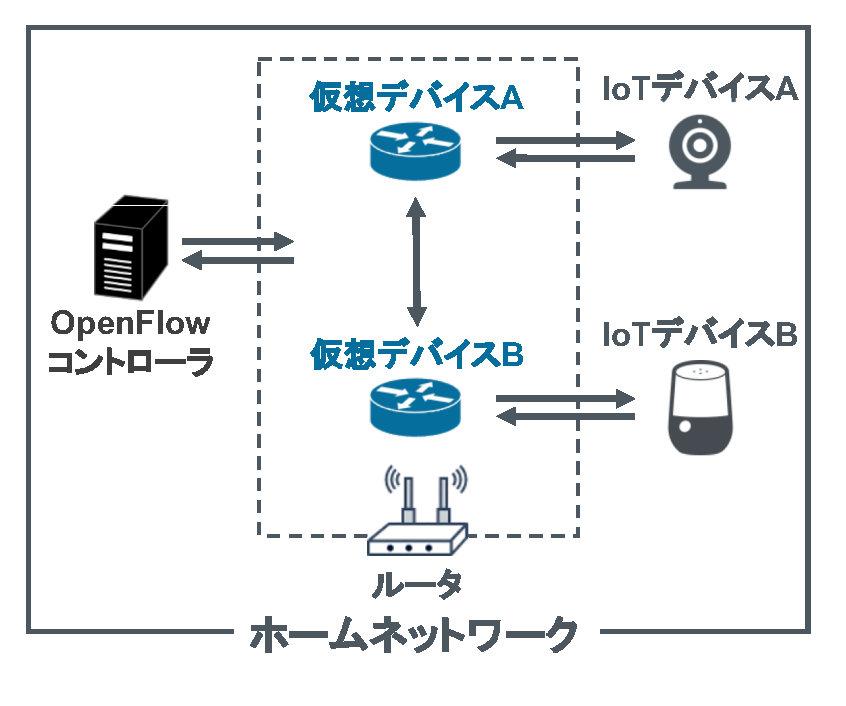
\includegraphics[width=\linewidth]{img/system.eps}
	\caption{提案システムの構成}
	\label{fig:system}
\end{figure}


\section{提案システム}
\subsection{概要}
本研究では,コンテナ上にセキュリティ対策を施したProxyを作成し,IoTデバイスに対してセキュリティ対策を適用するシステムを提案する.提案システムでは,IoTデバイスがリソース量の制限により適用できないセキュリティ対策をProxyにオフロードし,IoTデバイス間の通信を中継することで,本来IoTデバイスに適用したいセキュリティ対策を実現する.
また,OpenFlowの機能も追加し,ネットワークの監視を行う.ホームネットワーク内通信のトラフィック情報は既知であることを考慮し,フローの検証をOpenFlowコントローラで行う.
詳細なセキュリティ対策については後述する.


\subsection{システム構成}
提案システムの構成を図\ref{fig:system}に示す.本提案システムの構成要素は,IoTデバイス,Proxy,ルータ,OpenFlowコントローラから構成される.
\begin{itemize}
	\item \underline{IoTデバイス}\mbox{}\\
	      本研究で扱うIoTデバイスは,CPU等のリソースを十分に保持しておらず,直接セキュリティ対策を適用できないデバイスと定義する.
	\item \underline{Proxy}\mbox{}\\
	      IoTデバイスに要求されるセキュリティ対策を,仮想的に実現したものである.IoTデバイスからの通信を中継し,セキュリティ対策を適用する.各IoTデバイスに必要なセキュリティ対策をそれぞれ作成,適用することで,対象デバイスに応じた必要な対策を実現できる.
	\item \underline{ルータ}\mbox{}\\
	      IoTデバイス間通信の中継機器として用いる.ルータ上にProxyの実行環境を生成する.Proxyが作成される際に要求されるリソースを十分に提供することが可能とする.
	\item \underline{OpenFlowコントローラ}\mbox{}\\
	      Proxy内に作成されたOpenFlowスイッチと通信を行い,ホームネットワーク内の通信を監視する.ホームネットワーク内部に設置する.
\end{itemize}

\begin{figure}[!tb]
	\centering
	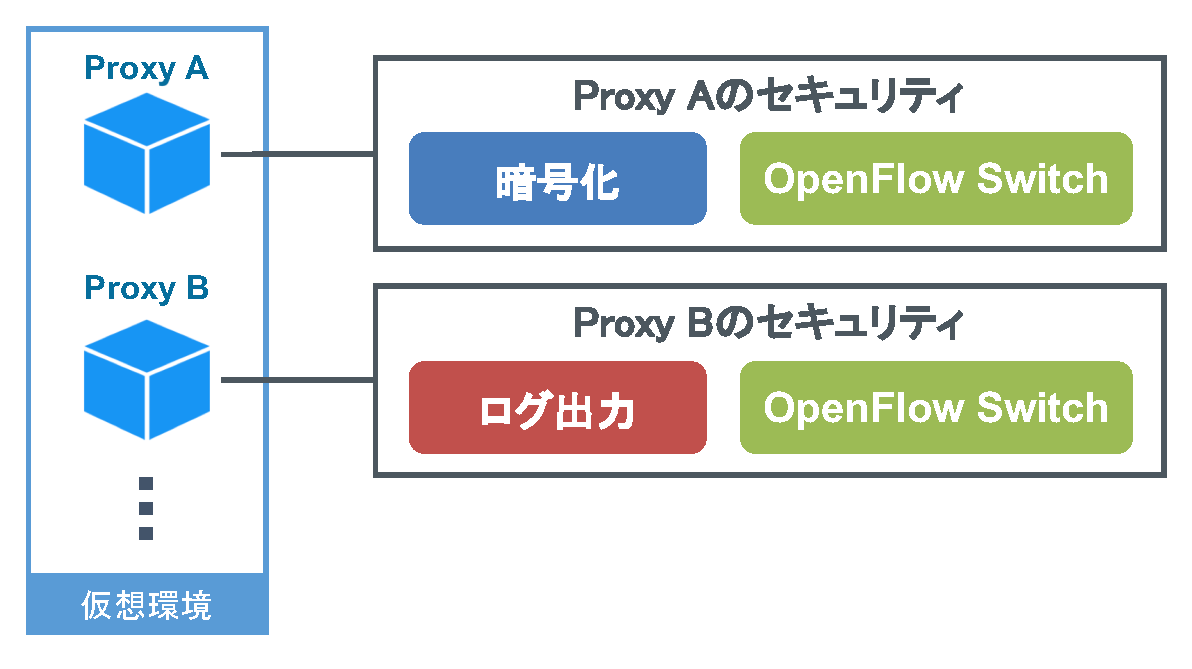
\includegraphics[width=\linewidth]{img/security.eps}
	\caption{Proxyのセキュリティ対策}
	\label{fig:security}
\end{figure}

\begin{figure}[!tb]
	\centering
	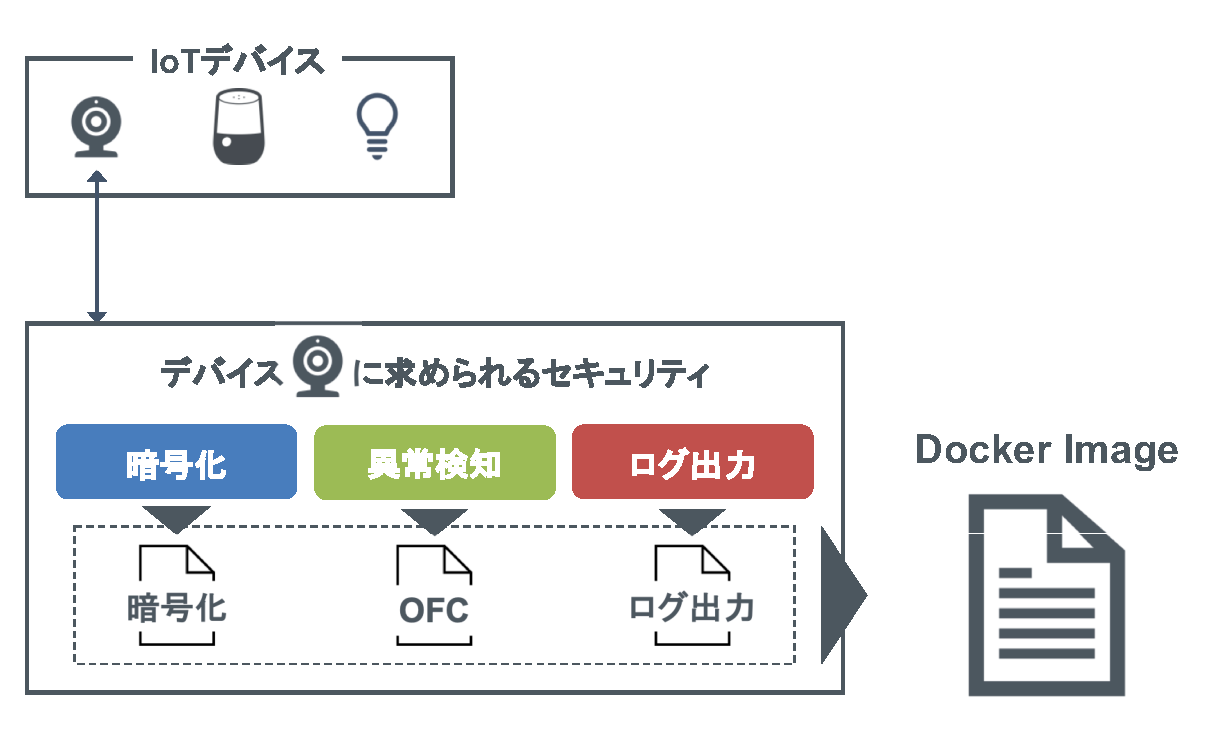
\includegraphics[width=\linewidth]{img/dockerimage.eps}
	\caption{imageファイルの作成}
	\label{fig:dockerimage}
\end{figure}

\subsection{Proxyのセキュリティ対策}
本研究におけるセキュリティ対策の特徴として,Proxyごとに異なるセキュリティ対策を適用可能なことが挙げられる.Proxyのセキュリティ対策の適用例を図\ref{fig:security}に示す.これにより,機能制限が原因でIoTデバイスに直接適用できないセキュリティ対策を導入できる.また,前述のホームネットワークの問題点で述べたような様々なハードウェアやアプリケーションへの適用や,様々なセキュリティ要件の変更に対しても柔軟に対応が可能となる.\par
また,コンテナ上で展開されるセキュリティ対策は,適応したいセキュリティ対策に対応したコンテナのimageファイルで定義される.imageファイルの作成図を図\ref{fig:dockerimage}に示す.この図のように,IoTデバイスに対して適用したいセキュリティが複数ある場合においても,対象デバイスの規格に対応した対策をそれぞれ作成し,ソフトウェアモジュールのような形で組み合わせて定義することで,imageファイルを作成することが可能となる.

\begin{figure}[!tb]
	\centering
	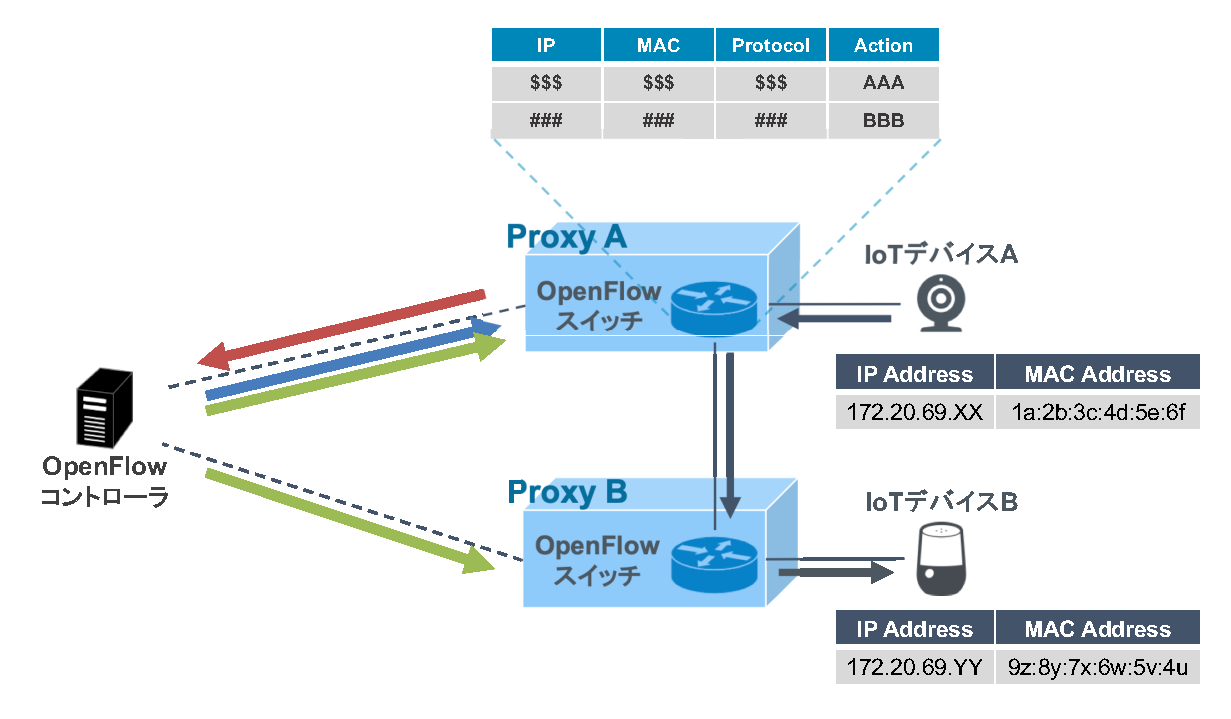
\includegraphics[width=\linewidth]{img/openflow.eps}
	\caption{OpenFlowにおけるフローチェック}
	\label{fig:openflow}
\end{figure}

\subsection{OpenFlowによるフローチェック}
本研究におけるネットワーク監視をOpenFlowを用いて行う.OpenFlowによるフローチェックを図\ref{fig:openflow}に示す.一つのIoTデバイスに対し,コンテナ上にOpenFlowスイッチの機能を生成する.IoTデバイスはこのOpenFlowスイッチを中継し,デバイス間通信を行う.OpenFlowコントローラは事前にIoTデバイスの情報を保持しており,OpenFlowスイッチとの通信が確立でき次第,デバイス間通信のフローテーブルを作成する.ホームネットワークの特性である各IoTデバイスのトラフィック情報は既知であり,変化が大きくないことを考慮し,IPアドレスや通信頻度の確認を行い,フローレベルにおける異常の検知を行う.異常を検知した場合は,そのパケットのDrop処理を指示したフローテーブルに変更し,その後フローテーブルを削除する.また同時に,ユーザへ異常検知を通知する.

\subsection{動作手順}
IoTデバイスの所有者であるユーザが本提案システムを利用する際の動作手順を図\ref{fig:seaquence}と以下に示す.
\begin{enumerate}
	\item ユーザは,デバイスをLAN内に接続した後,Proxyの実行環境へアクセスし,Proxyを作成するよう要求.
	\item 実行環境は,ホームネットワーク内にIoTデバイスが接続されたことを確認.
	\item 実行環境は,コンテナ共有サービスからimageファイルを取得.
	\item 取得したimageファイルを基に実行環境内にProxyを作成.
	\item Proxyは,デバイス情報を基にIoTデバイスに接続を行い,Proxyを経由して通信を行うように設定.
	\item Proxyは,OpenFlowコントローラへデバイス情報を送信.
	\item 実行環境は,Proxyの設定が完了し,IoTデバイス・Proxy間の通信が確立された後,Proxyの作成・ネットワークの監視状況を報告.
\end{enumerate}


\begin{figure}[!tb]
	\centering
	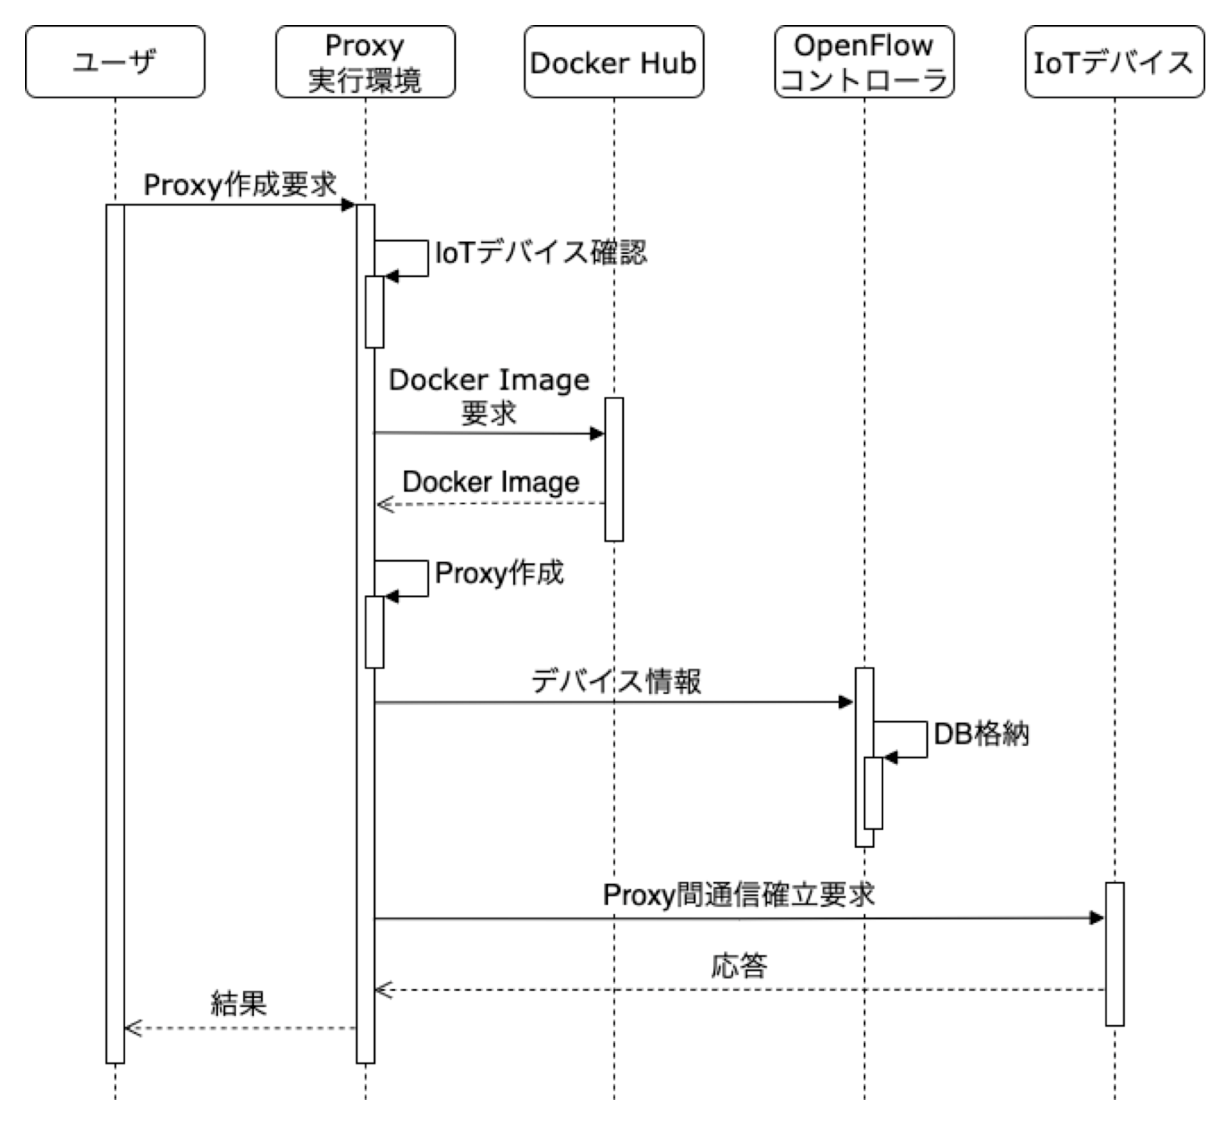
\includegraphics[width=\linewidth]{img/seaquence.eps}
	\caption{動作手順のシーケンス図}
	\label{fig:seaquence}
\end{figure}

\subsection{想定ユースケース}
本提案システムを用いた想定ユースケースを以下に示す.

\begin{itemize}
	\item \underline{セキュリティ対策を事前に提供する場合}\mbox{}\\
	      TLS/SSLによる通信の暗号化など,IoTデバイスのリソース制限により適用できないセキュリティ対策を事前にimageファイルとして提供し,Proxy上で実現する.
	\item \underline{インシデント発生時などに対策を提供する場合}\mbox{}\\
	      事前に提供していたセキュリティ対策では想定していなかったインシデントが発生した場合に,対象デバイスが保持するリソース量に依存せず,追加のセキュリティ対策を提供することが可能となる.
\end{itemize}

\section{シミュレーション実験}
\subsection{実装環境}
本研究の実装環境,実装環境の構成をそれぞれ表\ref{tab:program}と図\ref{fig:program}に示す.Proxyの作成方法としては,コンテナ仮想化を用いてアプリケーションを開発・実行するためのオープンプラットフォームであるDockerを利用した.Dockerで作成されるコンテナ上でProxyを稼働させることで,複数のProxyをリソースやオーバーヘッドを抑えて作成できる.また,これらのProxyは,Docker Hubより配布されるDocker Imageを用いることで容易に作成でき,コンテナをアップロードして公開・共有できる.また,OpenFlowコントローラは,SDNを実現するための開発フレームワークであるRyuを用いて作成した.
% また今回扱う通信プロトコルとしてはhttp(REST)を想定する.

\begin{table}[!tb]
	\caption{実装環境}
	\label{tab:program}
	\centering
	\begin{tabular}{c|l|l}
		\hline
		種類     & 項目       & 説明                  \\
		\hline \hline
		Proxy    & 使用ソフト & Docker                \\
		         & OS         & Ubuntu 20.04          \\
		         & CPU        & 3.60GHz Intel Core i9 \\
		         & メモリ     & 5GB                   \\
		\hline
		OpenFlow & 使用ソフト & Ryu                   \\
		         & OS         & Ubuntu 20.04          \\
		         & CPU        & 3.60GHz Intel Core i9 \\
		         & メモリ     & 5GB                   \\
		         & 使用言語   & Python                \\
		\hline
	\end{tabular}
\end{table}

\begin{figure}[!tb]
	\centering
	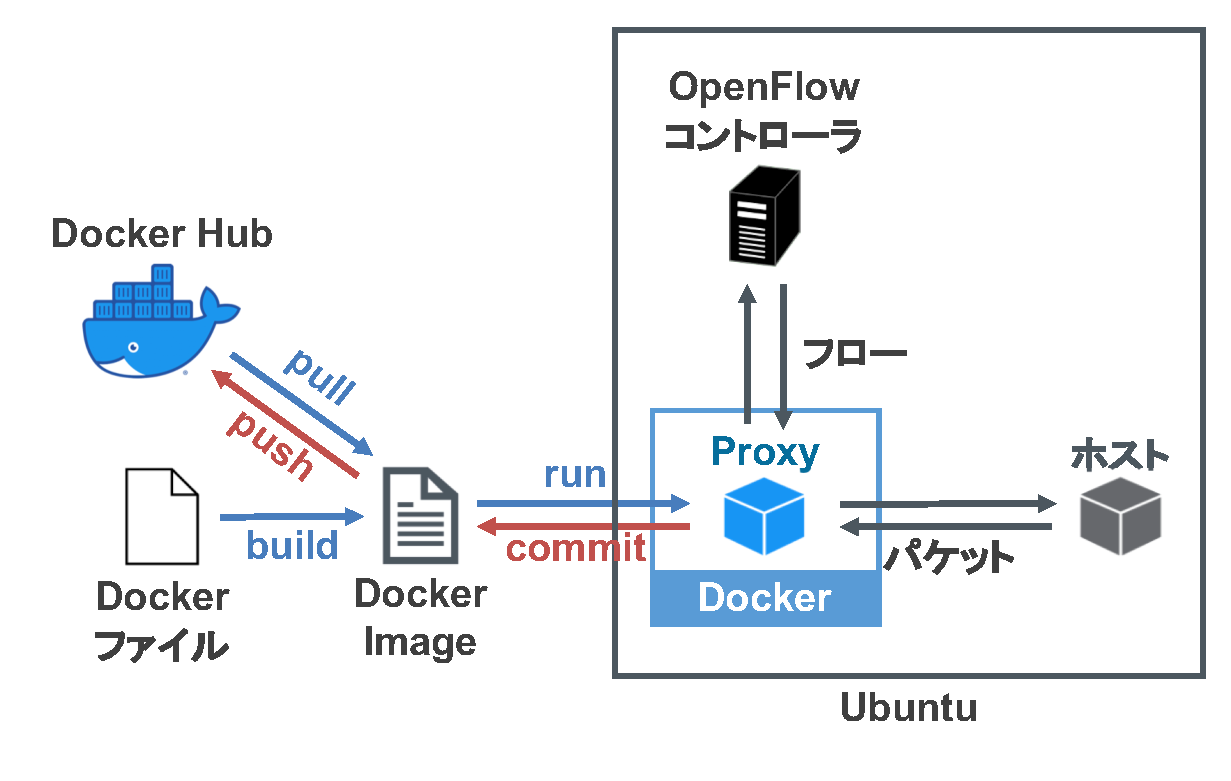
\includegraphics[width=\linewidth]{img/program.eps}
	\caption{実装環境の構成}
	\label{fig:program}
\end{figure}

\begin{figure*}[!tb]
	\centering
	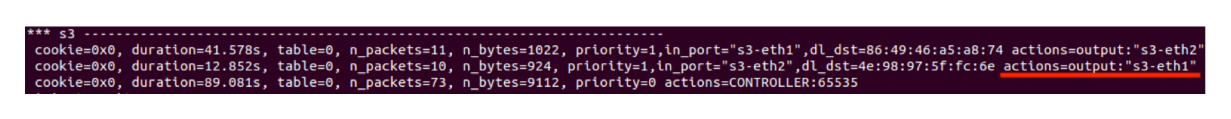
\includegraphics[width=\linewidth]{img/result_flow4v3.eps}
	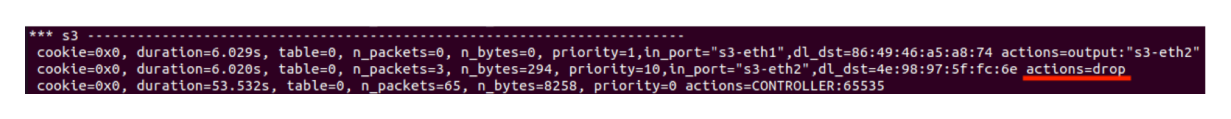
\includegraphics[width=\linewidth]{img/result_flow2v3.eps}
	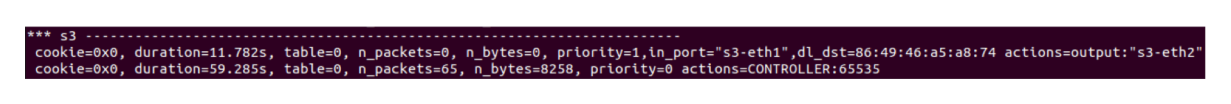
\includegraphics[width=\linewidth]{img/result_flow3v2.eps}
	\caption{登録済みのホストのフローテーブル(上),異常時のパケットをDrop処理するフローテーブル(中),その後のアクションが削除されたフローテーブル(下)}
	\label{fig:result1}
\end{figure*}

\subsection{評価内容}
本研究の評価として,まずセキュリティ対策が適用されているかを検証した.今回は登録されていないIoTデバイスから通信があった場合と,あるデイバイスからの通信頻度が通常と異なる場合を想定した.その状況において,コンテナ上で作成したOpenFlowによるフローチェックが行われているかを検証した.\par
また,提案システムの有効性を示すため,提案システムを適用した上で,IoTデバイス間通信を行なった際のラウンドトリップタイムの計測を行った.比較対象として,セキュリティ対策を適用せず,ルータを経由してデバイス間通信を行う場合についても計測を行った.ラウンドトリップタイムは,100回通信を行なった際の平均値を算出した.

\subsection{評価環境}
今回適用するセキュリティ対策としては,SSL/TLSプロキシによる暗号化のイメージをDocker Hubより取得し,適用した.また,OpenFlowスイッチのイメージも取得し,OpenFlowによるフローチェックも行った.事前に2台のホストを設置した環境に,新たに1台ホストを追加し,そのホストが通信要求を行う環境を作成した.


\section{結果と考察}
\subsection{評価結果}
登録済みのIoTデバイスから通信要求が来た場合,登録していないIoTデバイスや,通常の通信頻度と異なる等の異常の通信がなされている場合のフローテーブルの結果を図\ref{fig:result1}に示す.通常時は他のデバイスに対し,通信を許可するフローテーブルが作成されている.一方で,異常時はパケットをDrop処理するフローテーブルが作成されており,その後,そのフローテーブルが削除されていることがわかる.\par
また,セキュリティ対策を施した提案システムとセキュリティ対策を施してないシステムにおける通信の比較結果を図\ref{fig:result2}に示す.提案システムは,セキュリティ対策を施していないシステムにおける通信より,僅かであるがラウンドトリップタイムが劣っていることがわかる.

\subsection{信頼性に関する考察}
IoTデバイスを用いたシステムの安心安全を確保するための機能として,IPAによりIoT高信頼化機能が定義されている.IoT高信頼化要件として,開始,予防,検知,回復,終了の5つの局面に分けてそれぞれセキュリティ要件が定義されている\cite{IPA}.今回は前述の5つより,システム稼働中の局面である予防,検知,回復の3つにおける高信頼化要件に対し,提案システムの信頼性について考察する.

\begin{itemize}
	\item \underline{予防の局面における考察}\mbox{}\\
	      予防の局面での高信頼化要件は,稼働中の異常発生を未然に防止できることである.これに対応するIoT高信頼化機能としては,ログ取集機能,暗号化機能等があり,異常の予兆の把握,資産の保護を実現する.提案システムを用いることで,リソース量の制限により通常のIoTデバイスに適用できない機能であっても適用可能となる.
	\item \underline{検知の局面における考察}\mbox{}\\
	      検知の局面での高信頼化要件は,稼働中の異常発生を早期に検知できることである.これに対応するIoT高信頼化機能としては,OpenFlowによるネットワーク監視機能,ログ収集機能があり,以上発生の検知や発生原因の特定を実現する.提案システムを用いることで,予防の局面同様,デバイスのリソース量に依存せず,要求機能を実現できる.また,Proxyは各IoTデバイスごとに作成するため,個々のデバイスに応じた検知対策を適用可能となる.
	\item \underline{回復の局面における考察}\mbox{}\\
	      回復の局面での高信頼化要件は,異常が発生した場合に稼働の復旧ができることである.特にIoTでは,様々なデバイスが相互通信を行うため,事前に予測していなかった異常が発生することが想定される.今回の環境では,各セキュリティ対策はDocker HubからDockerイメージとして提供する.そのため,事前に作成したセキュリティ対策だけでなく,追加のセキュリティ対策も配布・適用が容易である.
\end{itemize}

\begin{figure}[!tb]
	\centering
	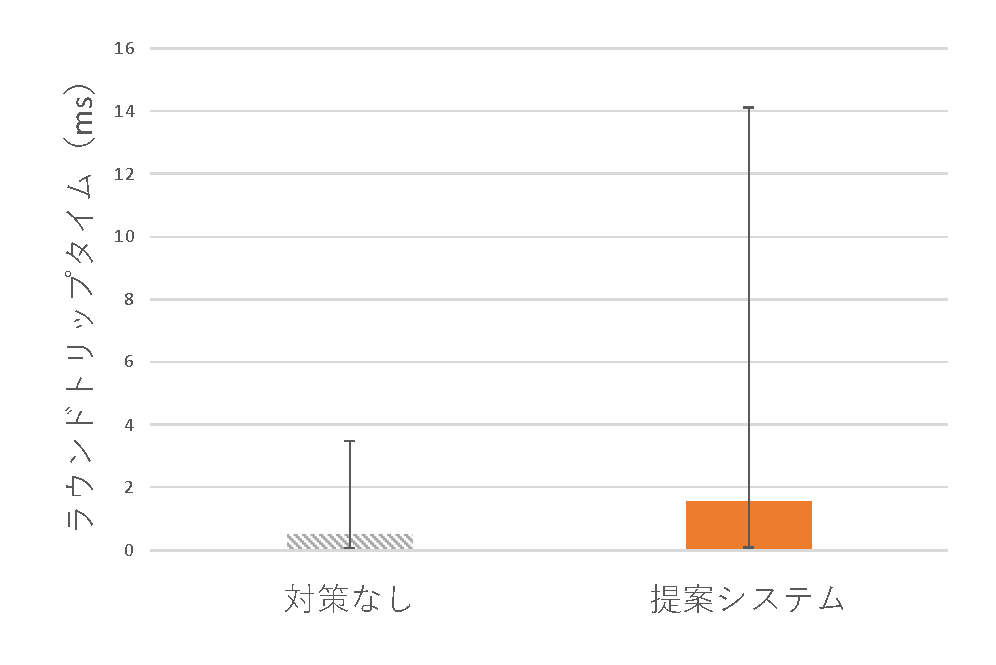
\includegraphics[width=\linewidth]{img/result.eps}
	\caption{IoTデバイス間通信の平均ラウンドトリップタイム}
	\label{fig:result2}
\end{figure}

\subsection{通信性能に関する考察}
図\ref{fig:result2}より,本提案システムは,セキュリティ対策なしの場合と比較し,遅延は発生している.しかし,約1msの違いであり,スマートハウス等の領域では遅延許容度が高いとされているため,許容範囲内であり,有用性がある.\par
今後,IoTデバイスが普及した際には,クラウドへの通信やデバイス間の通信が増加するため,帯域の輻輳や通信の干渉などの問題も発生すると予想される.そのため,通信遅延はさらに増加することが想定されることから,通信遅延の許容が難しいアプリケーションを利用する際にセキュリティ対策が必要な場合には,本提案システムが有効となる.

\section{まとめ}
本研究では,IoTのセキュリティ上のリスクにおいて,今後,ホームネットワーク内で閉じたデバイス間通信が多くなり,各IoTデバイスにおいてアクセス制御等の更なるセキュリティ対策を行う必要があることに注目した.
そこで,コンテナを用いたIoTデバイスへのセキュリティ対策の適用とOpenFlowを用いたホームネットワーク監視を行うフレームワークの構築を検討した.提案システムでは,コンテナ上にProxyを作成し,暗号化やOpenFlowスイッチ等のセキュリティ対策をオフロードし,IoTデバイス間の通信を中継することで,本来IoTデバイスに適用したいセキュリティ対策を実現した.
そして,IoTデバイス間で閉じた通信を行うシミュレーション評価の比較を行い,ホームネットワークにおいてセキュリティ要件を保つことと通信性能も許容範囲であることを示した.\par
今後は,オーケストレータ等を用いて,新しいIoTデバイスがホームネットワークに追加された際に,自動的にコンテナがProxyとして配備される仕組みを検討する.また,Raspberry Pi等の実機を用いた実験を行う予定である.

\begin{thebibliography}{10}
	\bibitem{security} 総務省, "IoT・5Gセキュリティ総合対策2020", サイバーセキュリティタスクフォース, pp.1-56, 2020.
	\bibitem{openflow} N. McKeown, T. Anderson, H. Balakrishnan, G. Parulkar, L. Peterson, J. Rexford, S. Shenker, and J. Turner, "OpenFlow: enabling innovation in campus networks", SIGCOMM Computer Communication Review, Vol.38, No.2, pp.69-74, 2008.
	\bibitem{camera} P. A. Abdalla and C. Varol, "Testing IoT Security: The Case Study of an IP Camera", 2020 8th International Symposium on Digital Forensics and Security (ISDFS), pp.1-5, 2020.
	\bibitem{owasp} P. Ferrara, A. K. Mandal, A. Cortesi and F. Spoto, "Static analysis for discovering IoT vulnerabilities", International Journal on Software Tools for Technology Transfer, Vol.23, No.1, pp.71-88, 2021.
	\bibitem{lowcost} A. Sivanathan, D. Sherratt, H. H. Gharakheili, V. Sivaraman and A. Vishwanath, "Low-cost flow-based security solutions for smart-home IoT devices," 2016 IEEE International Conference on Advanced Networks and Telecommunications Systems (ANTS), pp.1-6, 2016.
	\bibitem{d2d} P. Pawar and A. Trivedi, "Device-to-Device Communication Based IoT System: Benefits and Challenges", IETE Technical Review, Vol.36, No.4, pp.362-374, 2019.
	\bibitem{disap} M. Serror, M. Henze, S. Hack, M. Schuba, and K. Wehrle, "Towards In-Network Security for Smart Homes", Proceedings of the 13th International Conference on Availability, Reliability and Security (ARES 2018), No.18, pp.1-8, 2018.
	\bibitem{sover} Z. Zhang, T. Yu, X. Ma, Y. Guan, P. Moll and L. Zhang, "Sovereign: Self-contained Smart Home with Data-centric Network and Security", IEEE Internet of Things Journal, 2022.
	\bibitem{IPA} IPA技術本部 ソフトウェア高信頼化センター(SEC), "「つながる世界の開発指針」の実践に向けた手引き [IoT高信頼化機能編]", pp.1-96, 2017.
	\bibitem{latency} 総務省, "スマートIoT推進戦略", https://www.soumu.go.jp/main_content/000424359.pdf

\end{thebibliography}

\end{document}
